\section{Inledning}
Projektet ska utveckla ett system vilket styr bilar runt en bilbana efter en given referenstid. Till förfogande finns, en bilbana, ett antal bilar, en display samt en dator.
Målet med detta projekt är att bilarna skas köras runt banan inom 0,5 sekunder av den referenstid som användaren har angett. Efter en avslutad
körning på x varv ska standardaviklesen på varvtiderna inte överskrida 0,2 sekunder. Systemet skrivs i MatLab och har som huvudsyfte att reglera den spänning som bilbanan skickar
till bilarna. Olika bilar beter sig olika utifrån vissa skillnader bland bilarna, till exempel vikt, motorn i dem samt den magnet under bilarna som håller dem någorlunda fast på banan. 
Hela systemet ska styras utifrån en touch display som är enkel att förstå för gemene man och efter avslutad körning ska den även visa statistik om hur körningen gick. 
\begin{figure}
	\centering
	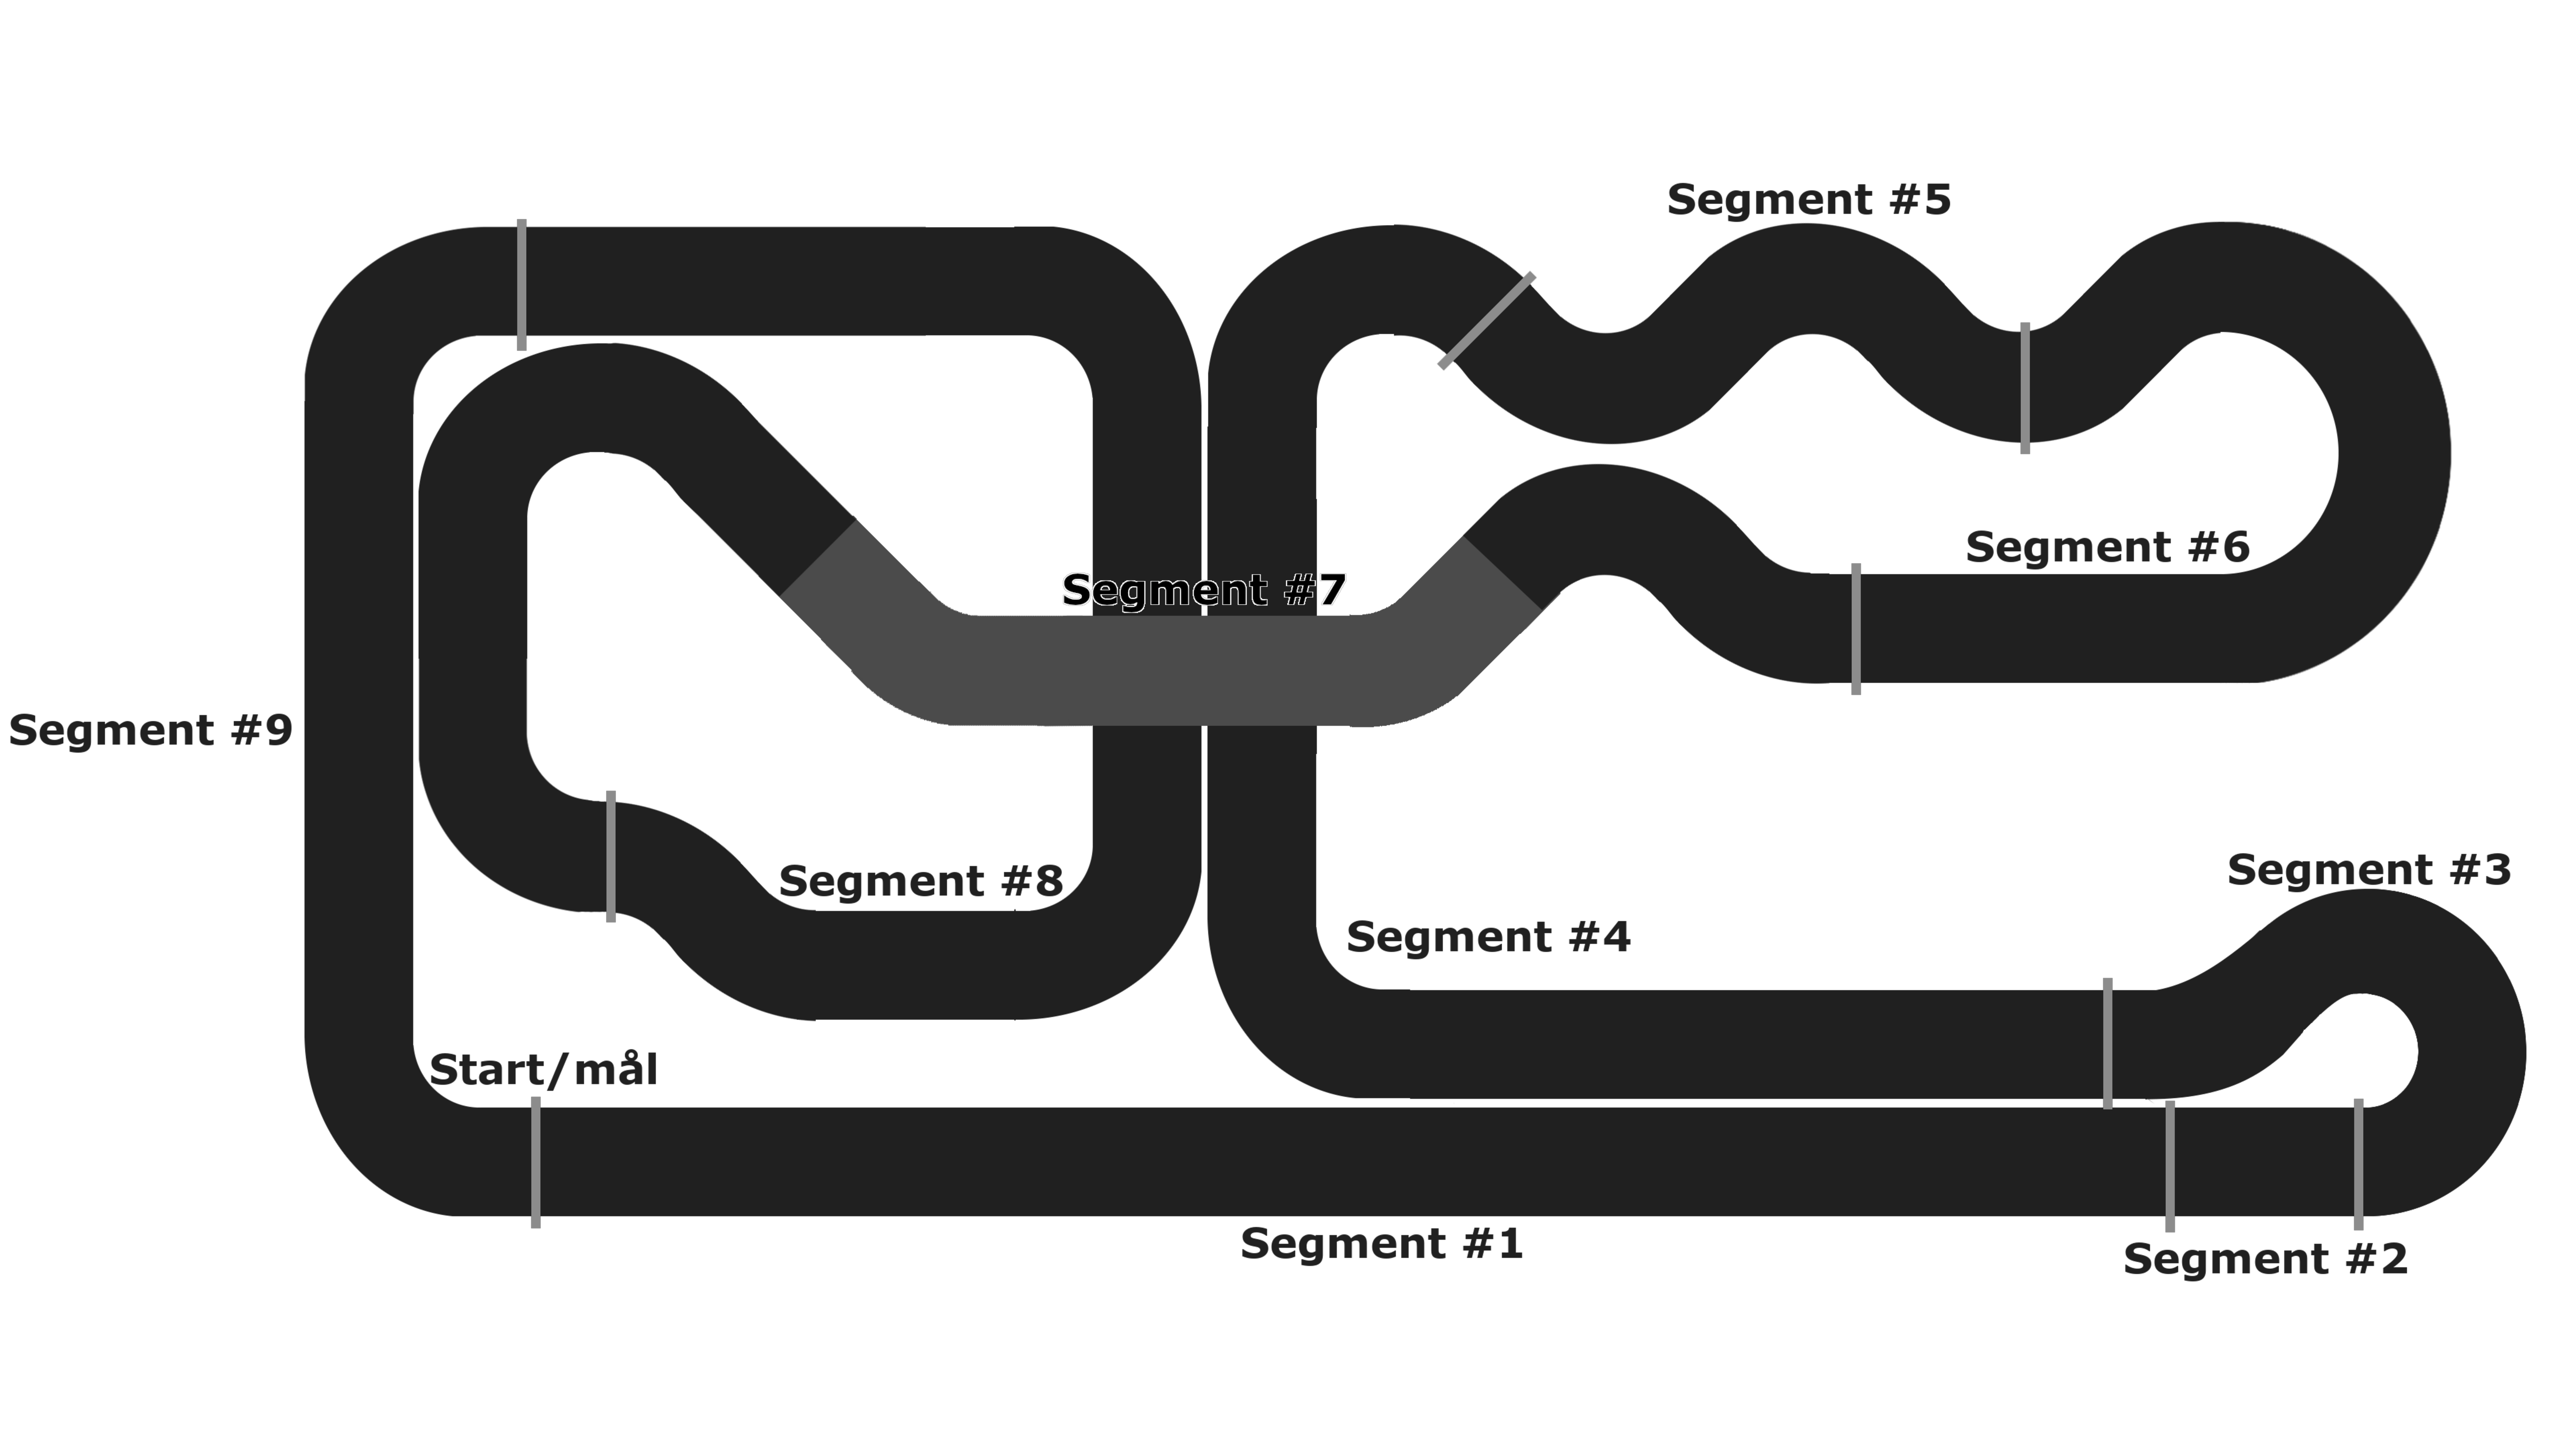
\includegraphics[width=\linewidth] {Figures/BanaModell}
	\caption{En modell av bilbanan.}
	\label{fig:bilbanan}
\end{figure}

\subsection{Bakgrund} 

Projektet har utförts med hjälp av en bilbana samt flera bilar, givare,
spänningsaggregat och två datorer inne i bilbanerummet. Via datorn har spänning
tillförts till bilbanan. Med hjälp av givarna är det möjligt att veta när en bil
har passerat en givare. Programvaran har utvecklats i Matlab.

\subsection{Syfte och mål}

Syftet med projektet är att lära sig att arbeta i ett projekt utifrån
projektstyrningsmodellen LIPS. Målet med projektet var att konstruera ett system
som kunde köra bilar runt en bilbana på en vald referenstid mellan 12 och 15
sekunder. Detta skulle göras för flera bilar med olika egenskaper. Fler krav som
ska klaras av finns i kravspecifikationen (\ref{app:kravbeskrivning}).

\subsection{Avgränsningar}

- Ingen gemensam målgång
